\section{Aufbau}
\label{sec:Aufbau}

Der Aufbau der Apparatur ist in Abbildung \ref{fig:Aufbau} zu sehen.
Ein mit $\mathrm{Sr}^{2+}$-Ionen versetzter KBr-Kristall befindet sich in einem Gefäß, welches mit einer Vakuumpumpe verbunden ist und dessen Innendruck $p\approx\SI{E-2}{\milli\bar}$ beträgt. Der untere Teil ist mit einer Heizstromquelle verbunden und verfügt über einen Kühlfinger aus gut wärmeleitendem Kupfer.
Der Deckel und der Boden des wärmeisolierten Behälters besteht aus einem Plattenkondensator, der mit einem Gleichspannungsnetzgerät, einem Kabel zum entladen und einem Piccoamperemeter verbunden werden kann.

\begin{figure}
	\centering
	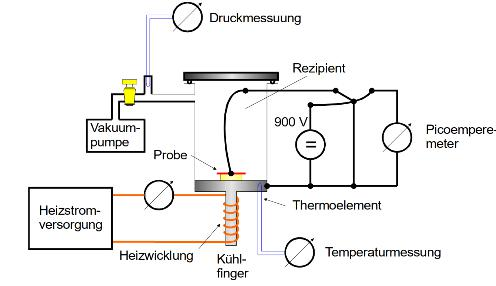
\includegraphics[width=\linewidth-70pt,height=\textheight-70pt,keepaspectratio]{content/images/Aufbau.jpg}
	\caption{Schematischer Aufbau des Versuchs \cite{V48}.}
	\label{fig:Aufbau}
\end{figure}
